Suppose we have a convex optimization problem where the objective function $f_0$ is differentiable. Let $X$ be the feasible set of the problem. Then $x \in X$ is optimal if and only if:

\begin{equation}
    \nabla f_0(x)^T(y-x) \geq 0 \quad \forall y \in X
\end{equation}

Geometrically, this means that the gradient of the objective function at $x$ points in the direction of the feasible set, in other words, it is a supporting hyperplane to $X$.

\begin{center}
    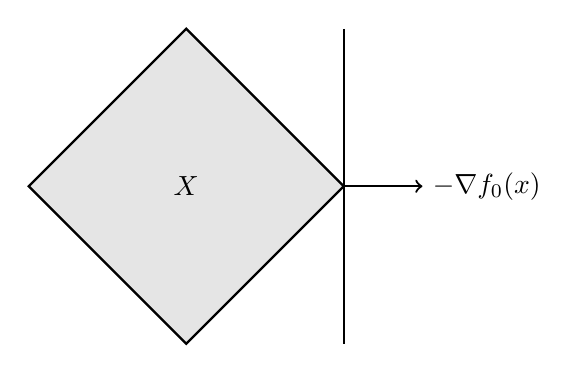
\begin{tikzpicture}[scale=2]
        % Define the convex set X
        \filldraw[fill=gray!20, draw=black] (-1,0) -- (0,1) -- (1,0) -- (0,-1) -- cycle;
        \draw[thick] (-1,0) -- (0,1) -- (1,0) -- (0,-1) -- cycle;

        % Define the tangent line and arrow
        \draw[thick] (1.0,1.0) -- (1.0,-1.0);
        \draw[->,thick] (1.0,0.0) -- (1.5,0.0) node[right]{$-\nabla f_0(x)$};

        % Add the name X to the set
        \node at (0,0) {$X$};
    \end{tikzpicture}
\end{center}

